\chapter{\ifproject%
\ifenglish Experimentation and Results\else การทดลองและผลลัพธ์\fi
\else%
\ifenglish System Evaluation\else การประเมินระบบ\fi
\fi}

เนื่องจากมีการนำความรู้เรื่อง Computer Vision มาใช้เกี่ยวกับการทำ Object detection จึงได้มีการศึกษา model และ library
ของ OpenCV ที่มีให้ทดลองใช้งาน เพื่อเพิ่มความเข้าใจและเลือกใช้ได้อย่างเหมาะสม โดยนำภาพบางส่วนจากการถ่ายรูปสถานที่จริงด้วยกล้องโทรศัพท์มือถือ คือบริเวณชั้น 2
ของสำนักหอสมุดมหาวิทยาลัยเชียงใหม่มาทำการทดสอบ ซึ่งผลลัพธ์ที่ได้มีดังนี้


\section{การทดลองครั้งที่ 1 โดยใช้ OpenCV DNN with TensorFlow}

% 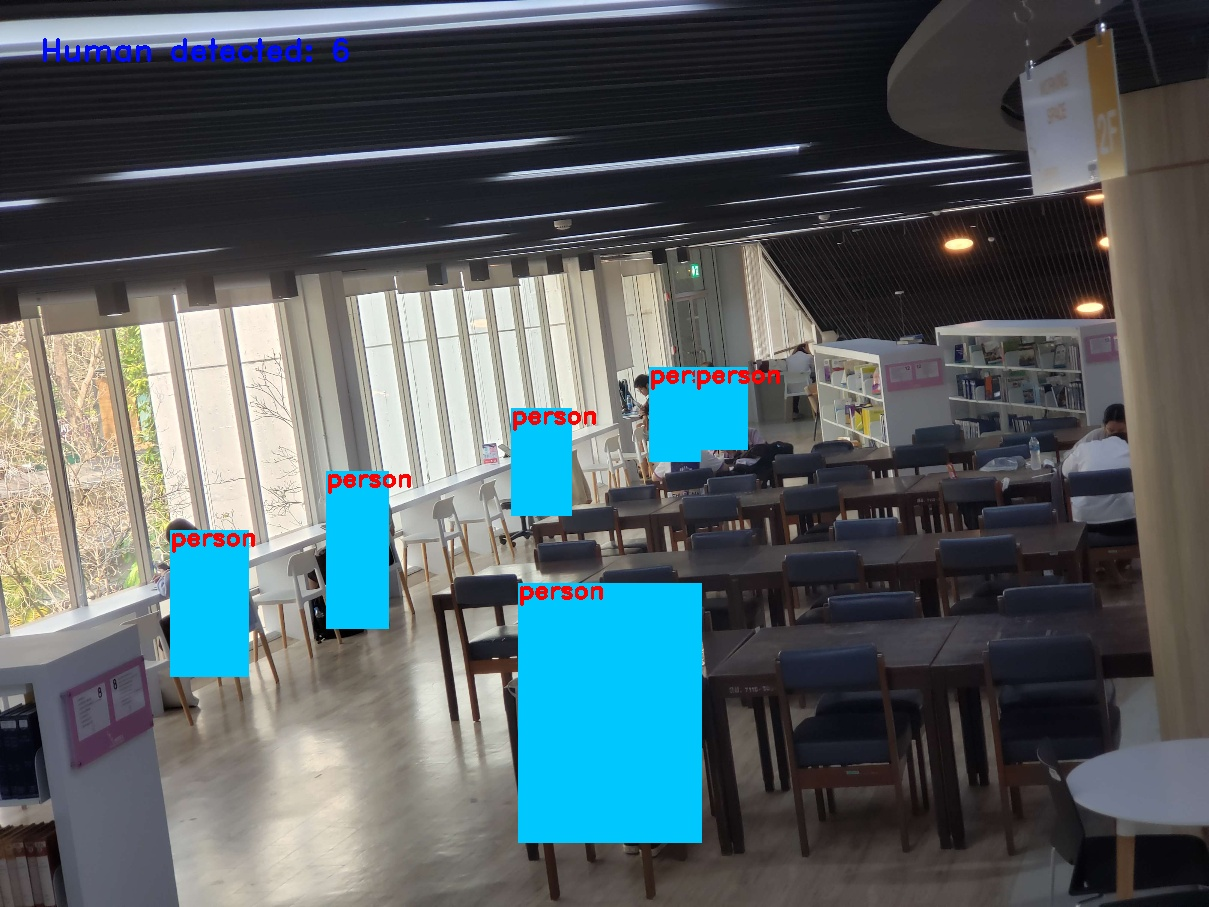
\includegraphics[width=\textwidth]{\images\output.jpg}
